%===================================== CHAP 6 =================================

\chapter{Testing}
The goal is to deliver a product with high quality and works according to the given requirements. Therefor the group aims to test most parts of the product, using different types of test methods. These methods are unit testing, integration testing, system testing and acceptance testing.


\section{Test strategy}
The group aims to use the pyramid testing model, see figure \ref{pyramid testing model}. This model contains many automated tests, this includes unit and integration tests. The model aims for many automated tests and a few graphical user interface (denoted as GUI) tests. This is because automated tests can run every time a new feature is added, but it takes more time to test the GUI for every new feature. GUI tests are more used later in the process, it is typical to include users in this testing process.

\begin{figure}[!ht]
    \centering
        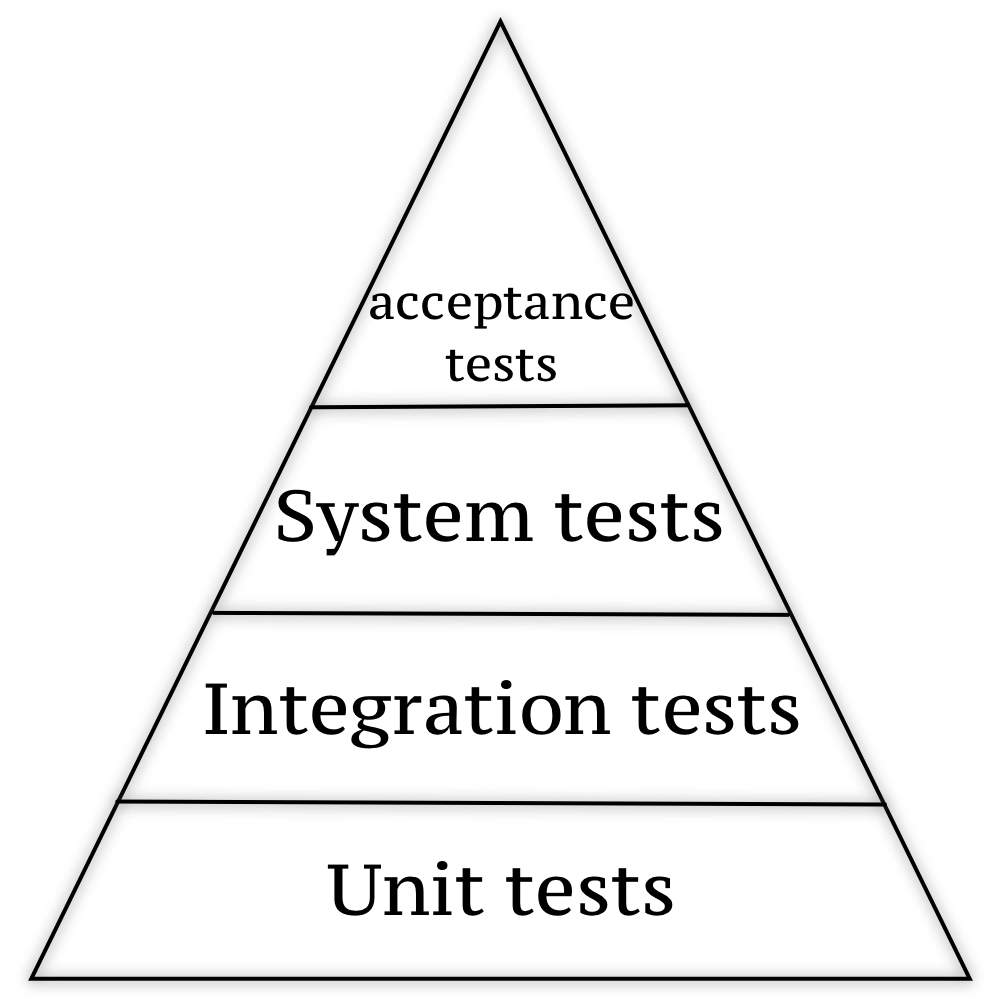
\includegraphics[width=0.3\textwidth]{fig/testpyramid}
    \caption{Pyramid testing model}
    \label{pyramid testing model}
 \end{figure}

\subsection{Test plan}
The group decided to create a test plan, see table \ref{Test plan}  to get an overview of what types of tests were to be performed during the project and to what time.

The customer wanted to include the users as much as possible during the development process. This was done to get feedback on the usability and the functionality. Therefore the test plan includes the acceptance tests, where the users needs and requirements are tested. The acceptance tests are based on the user cases, see chapter \ref{User cases}.

\begin{longtable}{|l|l|}
\hline
\rowcolor{Gray}
\textbf{Dates} & \textbf{Test cases to be tested} \\
\hline
13.03 - 17.03 (Sprint 3) & UCXX, UCXX,   \\
\hline
20.03 - 24.03 (Sprint 3) & Workshop with users, free testing\\
\hline
24.04 (Sprint 5) & All test cases \\
\hline
15.05 - 19.05 (Sprint 7) & Final test, test all cases  \\
\hline
\caption{Test plan}
\label{Test plan}
\end{longtable}


\subsection{Unit Testing}

\subsection{Integration Testing}

\subsection{System Testing}

\subsection{Acceptance Testing}
acceptance testing: Formal testing with respect to user needs, requirements, and business processes conducted to determine  whether or not a system satisfies the acceptance criteria and to enable the user, customers or other authorized entity to determine whether or not to accept the system. \cite{acceptanceTesting}

\subsubsection{Test cases}


\section{Test Execution}
\subsection{Unit Testing}

\subsection{Integration Testing}

\subsection{System Testing}

\subsection{Acceptance Testing}

\cleardoublepage